
In this section a step by step approach to reveal inner structures of a mesh will be discussed. First a plane needs to be defined that represents the position and direction of the cut. To retain interactivity, parameters in the VolumeShop interface are available to translate, rotate and scale the plane. The color and opacity of the plane should be adaptable to not occlude parts of the mesh. For the mesh splitting an offset is defined that indicates how far the two halves of the mesh shall be apart from the plane. The larger the gap the better the insight into the model. The splitting itself is no real translation of the two halves, but the model is rendered twice at different positions in space parallel to the plane. Respectively, the fragments on the other side of the plane are discarded and not rendered to create the illusion that the mesh has been split. After the cut, the back facing triangles become visible in those areas where the model has been cut. Therefore, the final step is shading these back faces to create shading for the cut surface.

\section{Definition of the plane}
\label{chap:planeDefinition}
The cutting plane to calculate the cut is defined by a point on the plane and a normal vector. Its dimension is per definition indefinite. Visually, the plane is represented as a rectangle with a certain user-defined dimension that is adaptable to the size of the mesh to be split. This gives the user an idea where the cut in the mesh is performed. Additionally, to increase comprehension for the user, the color of the plane, its opacity and scaling factor can be set by the user. The orientation of the cutting plane can be defined with properties like translation and rotation vectors that influence the calculation of the mesh splitting directly (cf. Algorithm~\ref{alg:initProperty}). To apply changes made in the interface immediately, an observer for the property has to be added (cf. Algorithm~\ref{alg:addObserverToProperty} and Chapter~\ref{chap:observers}).
\begin{algorithm}
\FuncSty{GetPlugin().GetProperty(\ArgSty{"Plane Translation"}).require(\ArgSty{Variant::TypeVector(Vector(0.0f, 0.0f, 0.0f))})}\;
\BlankLine
\caption{Property for translation of the plane named \emph{Plane Translation} of the type \emph{Vector} with a default value of \emph{(0.0, 0.0, 0.0)}. Defining a name and a type for a property is mandatory.}
\label{alg:initProperty}
\end{algorithm}
%\begin{lstlisting}
%GetPlugin().GetProperty("Plane Translation Vector").require(Variant::TypeVector(Vector(0.0f, 0.0f, 0.0f)));
%\end{lstlisting}

\begin{algorithm}
\FuncSty{GetPlugin().GetProperty(\ArgSty{"Plane Translation"}).addObserver(\ArgSty{\&m\_modVariantObserver})}\;
\BlankLine
\caption{Adding an observer to the property \emph{Plane Translation}.}
\label{alg:addObserverToProperty}
\end{algorithm}
%\begin{lstlisting}
%GetPlugin().GetProperty("Plane Translation Vector").addObserver(&m_modVariantObserver);
%\end{lstlisting}

Before drawing the plane, the \emph{Viewing Transformation Matrix} is loaded. This matrix is for transforming the coordinates from world space into viewing space~\cite{book:computerGraphicsHearn}. Then the plane is adjusted by its affine transformations (cf. Algorithm~\ref{alg:adjustPlane}). All parameters passed are of the type \texttt{float} and taken from the user input.
\LinesNumbered
\begin{algorithm}
\FuncSty{glTranslatef(\ArgSty{planeTranslation.GetX(), planeTranslation.GetY(), planeTranslation.GetZ()})}\;\label{ln:translation}
\FuncSty{glRotatef(\ArgSty{planeRotationAngle, planeRotation.GetX(), planeRotation.GetY(), vecPlaneRotation.GetZ()})}\;\label{ln:rotation}
\FuncSty{glScalef(\ArgSty{planeScaling.GetX(), planeScaling.GetY(), planeScaling.GetZ()})}\;\label{ln:scale}
\BlankLine
\caption{OpenGL commands for translating (cf. Line~\NlSty{\ref{ln:translation}}), rotating (cf. Line~\NlSty{\ref{ln:rotation}}) and scaling (cf. Line~\NlSty{\ref{ln:scale}}) the plane. These OpenGL commands do not accept vectors as parameters, hence the x-, y- and z-coordinates are taken from each property respectively and handed over as floating point values.}
\label{alg:adjustPlane}
\end{algorithm}
\LinesNotNumbered
%\begin{lstlisting}
%glTranslatef(vecPlaneTranslation.GetX(), vecPlaneTranslation.GetY(), vecPlaneTranslation.GetZ());
%glRotatef(vecPlaneRotationAngle, vecPlaneRotation.GetX(), vecPlaneRotation.GetY(), vecPlaneRotation.GetZ());
%glScalef(vecPlaneScaling.GetX(), vecPlaneScaling.GetY(), vecPlaneScaling.GetZ());
%\end{lstlisting}

The color of the plane is handed over from the input panel, normalized, and passed on to the renderer. An example for achieving this in VolumeShop is shown in Algorithm~\ref{alg:planeColor}.
\begin{algorithm}
\FuncSty{glColor4f(\ArgSty{planeColor.GetNormalizedRed(), planeColor.GetNormalizedGreen(), planeColor.GetNormalizedBlue(), planeColor.GetNormalizedAlpha()})}\;
\BlankLine
\caption{The individual color channels are taken from the user-defined input vector and used as input parameters for the OpenGL command \texttt{glColor4f}.}
\label{alg:planeColor}
\end{algorithm}
%\begin{lstlisting}
%glColor4f(vecPlaneColor.GetNormalizedRed(), vecPlaneColor.GetNormalizedGreen(), vecPlaneColor.GetNormalizedBlue(), vecPlaneColor.GetNormalizedAlpha());
%\end{lstlisting}

OpenGL supports several basic graphics primitives by default~\cite{book:computerGraphicsHill}. For the purpose as a visual helper the plane is displayed as a square with side length two. Note that the plane is also scalable to account for meshes of various sizes. The commands for drawing the square are shown in Algorithm~\ref{alg:openGlQuad}. Figure~\ref{fig:plane} shows a few examples of possible plane positions. 
\begin{algorithm}
\FuncSty{glBegin(\ArgSty{GL\_QUADS})}\;
\Indp\FuncSty{glNormal3f(\ArgSty{0, 0, 1})}\;
\FuncSty{glVertex3f(\ArgSty{-1, -1, 0})}\;
\FuncSty{glVertex3f(\ArgSty{1, -1, 0})}\;
\FuncSty{glVertex3f(\ArgSty{1, 1, 0})}\;
\FuncSty{glVertex3f(\ArgSty{-1, 1, 0})}\;
\Indm\FuncSty{glEnd()}\;
\BlankLine
\caption{A quad primitive with side length \emph{2} and depth \emph{0}.}
\label{alg:openGlQuad}
\end{algorithm}
%\begin{lstlisting}
%glBegin(GL_QUADS);
	%glNormal3f(0, 0, 1);
	%glVertex3f(-1, -1, 0);
	%glVertex3f( 1, -1, 0);
	%glVertex3f( 1,  1, 0);
	%glVertex3f(-1,  1, 0);
%glEnd();
%\end{lstlisting}

\begin{figure}%
\centering
\vspace{5.00mm}
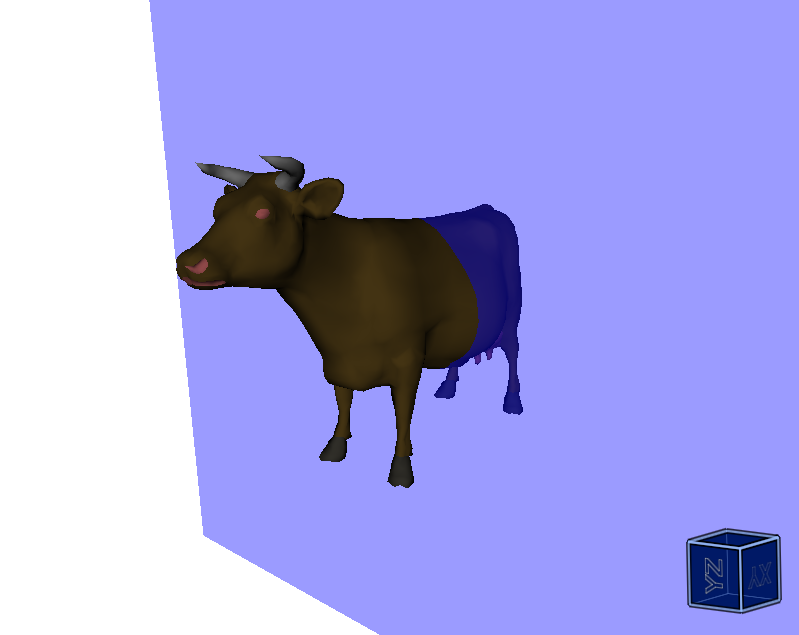
\includegraphics[width=0.3\textwidth]{ownChapters/figures/planeRotate90_010.png}%
\hspace{5.00mm}
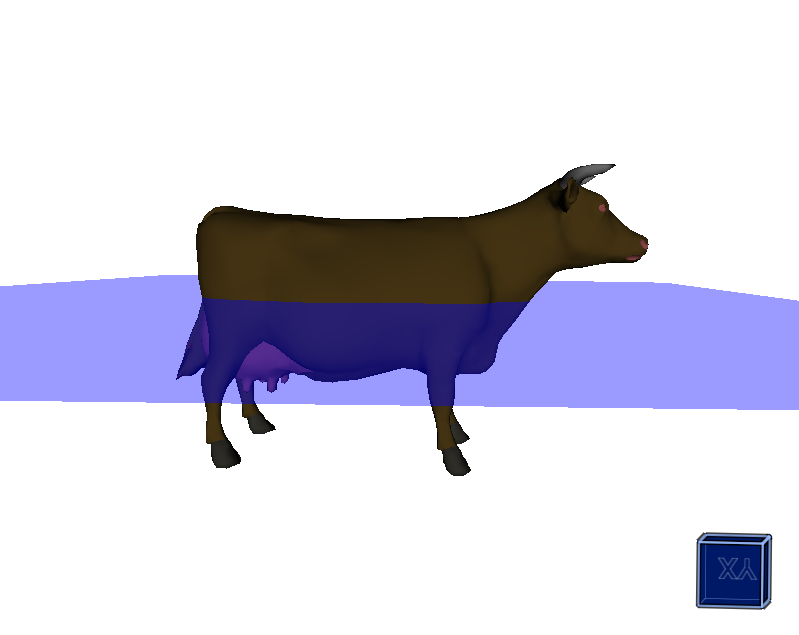
\includegraphics[width=0.3\textwidth]{ownChapters/figures/planeRotate90_100.png}%
\hspace{5.00mm}
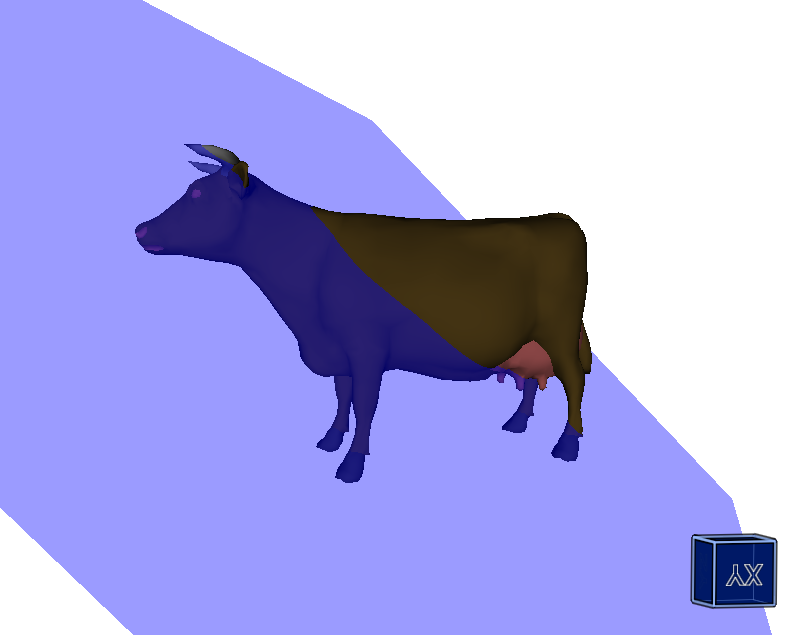
\includegraphics[width=0.3\textwidth]{ownChapters/figures/planeRotate90_101.png}%
\caption{Example of a plane with a different rotation of the normal vectors. The vectors from left to right: \emph{(0,1,0)}; \emph{(1,0,0)}; \emph{(1,0,1)}.}%
\label{fig:plane}%
\end{figure}

\section{Splitting the mesh}
The splitting offset is implemented as an VolumeShop user interface parameter. If the parameter is set to zero the mesh does not seem to be split, although it is still rendered twice. The larger the value of the offset the bigger the distance between the two halves of the mesh. An observer for the offset needs to be added as well (cf. Chapter~\ref{chap:observers} and Chapter~\ref{chap:planeDefinition}).

\subsection{Rotation of the planes' normal vector}
The normal of the plane has been defined as \texttt{(0.0,0.0,1.0)}, but regarding that the normal vector is still located in the object space of the plane, it needs to be transformed into the same space as the mesh. This is being done by rotating the normal by the same amount as the plane is rotated in the interface (cf. Algorithm~\ref{alg:rotation}).
\begin{algorithm}
\FuncSty{glRotatef(\ArgSty{rotationAngle, rotationVector.GetX(), rotationVector.GetY(), rotationVector.GetZ()})}\;
\BlankLine
\caption{The user-defined properties \emph{rotation angle} and \emph{rotation vector} reveal the rotation matrix.}
\label{alg:rotation}
\end{algorithm}
%\begin{lstlisting}
%glLoadIdentity();
%glRotatef(vecPlaneRotationAngle, vecPlaneRotationVector.GetX(), vecPlaneRotationVector.GetY(), vecPlaneRotationVector.GetZ());
%\end{lstlisting}

The rotation matrix could also be calculated using the generally known formulas~\cite{book:computerGraphicsHill}:\\%p217

x-roll:
\begin{equation}
R_{x}(\beta) = 
\begin{pmatrix} 
	1 & 0 & 0 & 0 \\ 
	0 & \cos(\beta) & -\sin(\beta) & 0 \\ 
	0 & \sin(\beta) & \cos(\beta) & 0 \\ 
	0 & 0 & 0 & 1 
\end{pmatrix}
\end{equation}

y-roll:
\begin{equation}
R_{y}(\beta) =
\begin{pmatrix} 
	\cos(\beta) & 0 & \sin(\beta) & 0 \\
	0 & 1 & 0 & 0 \\
	-\sin(\beta) & 0 & \cos(\beta) & 0 \\
	0 & 0 & 0 & 1
\end{pmatrix}
\end{equation}

z-roll:
\begin{equation}
R_{z}(\beta) =
\begin{pmatrix} 
	\cos(\beta) & -\sin(\beta) & 0 & 0 \\
	\sin(\beta) & \cos(\beta) & 0 & 0 \\
	0 & 0 & 1 & 0 \\
	0 & 0 & 0 & 1
\end{pmatrix}
\end{equation}

% book p 220
It should be considered that 3D rotation matrices do not commute~\cite{book:computerGraphicsHill}, so the order of multiplication matters. Subsequently, the rotated normal vector is multiplied with the model view matrix to transform the vector in model view space before it is normalized. After normalization the normal vector has a value between 0 and 1 (cf. Algorithm~\ref{alg:planeNormalization}).
\begin{algorithm}
\ArgSty{planeNormal}\FuncSty{.normalize()}\;
\BlankLine
\caption{Normalizing the plane normal}
\label{alg:planeNormalization}
\end{algorithm}
%\begin{lstlisting}
%planeNormal.normalize();
%\end{lstlisting}

\subsection{Translating the mesh}
The mesh is translated by an offset in the direction of the normal vector. The command in OpenGL for translation is \texttt{glTranslatef}. Before the mesh is rendered the shader needs to be bound.
\LinesNumbered
\begin{algorithm}
\FuncSty{Vector} \ArgSty{meshTranslation} = \ArgSty{planeNormal $\cdot$ offset}\;\label{ln:translationValue}
\FuncSty{glTranslatef(\ArgSty{meshTranslation.GetX(), meshTranslation.GetY(), meshTranslation.GetZ()})}\;\label{ln:mtranslation}
\ArgSty{m\_shaShader}\FuncSty{.bind()}\;\label{ln:bindShader}
\FuncSty{renderMesh(\ArgSty{*pMesh})}\;\label{ln:renderMesh}
\ArgSty{m\_shaShader}\FuncSty{.release()}\;\label{ln:releaseMesh}
\BlankLine
\caption{The value of the mesh translation is defined (cf. Line~\NlSty{\ref{ln:translationValue}}). Afterwards, the translation is applied (cf. Line~\NlSty{\ref{ln:mtranslation}}). Before rendering the mesh (cf. Line~\NlSty{\ref{ln:renderMesh}}), the shader needs to be bound (cf. Line~\NlSty{\ref{ln:bindShader}}).}
\label{alg:shaderBinding}
\end{algorithm}
\LinesNotNumbered
%\begin{lstlisting}
%Vector meshTranslation = planeNormal * offset;
%glTranslatef(meshTranslation.GetX(), meshTranslation.GetY(), meshTranslation.GetZ());
%m_shaShader.bind();
%renderMesh(*pMesh);
%m_shaShader.release();
%\end{lstlisting}

As stated previously, the mesh is rendered twice to create the illusion of a mesh that is dragged apart. Therefore, the mesh needs to be rendered again with a translation in the opposite direction. In VolumeShop, the two meshes are displayed with a plane in between. The distance of the meshes is twice the offset (cf. Figure~\ref{fig:offset}).

\begin{figure}%
\centering
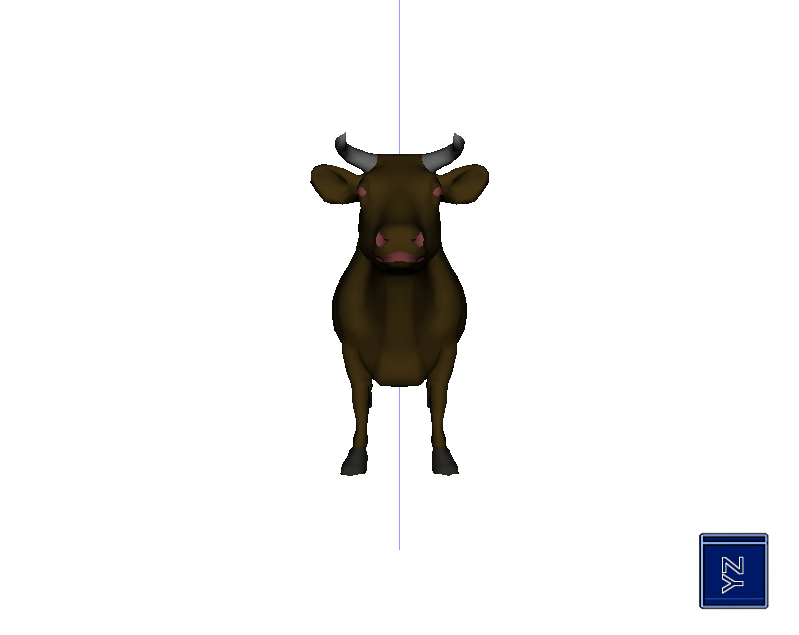
\includegraphics[width=0.4\textwidth]{ownChapters/figures/1_noOffset.png}%
\hspace{7.00mm}
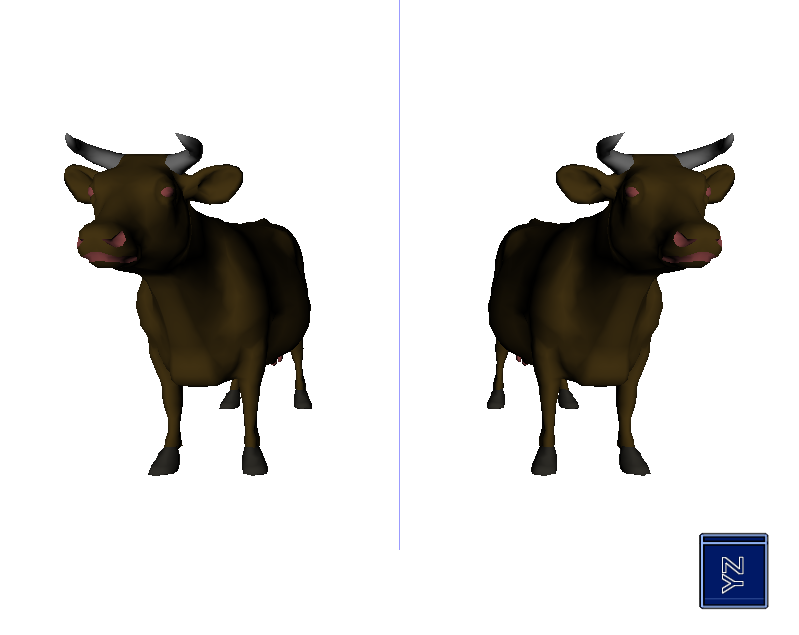
\includegraphics[width=0.4\textwidth]{ownChapters/figures/2_offset.png}%
\caption{The mesh with no offset (left) and with offset applied (right)}%
\label{fig:offset}%
\end{figure}

\subsection{Discarding dispensable fragments}
To eliminate the pixels from the other side of the plane of each mesh respectively, it has to be determined on which side of the plane a pixel lies. The computation is performed in the fragment shader (cf. Algorithm~\ref{alg:pointBeforePlane}).

\begin{algorithm}
\If{(N $\cdot$ (v - p)) $<=$ $0.0$} {\FuncSty{discard}\;}
\caption{The dot product of the plane normal \emph{N} and the vertex position \emph{v} subtracted by a point on the plane \emph{p} states if the vertex is in front of or behind the cutting plane. A value greater than zero states that the point is in front of the plane. In case the point is behind the plane, it is discarded.}
\BlankLine
\label{alg:pointBeforePlane}
\end{algorithm}

Before the mesh is rendered, the normal of the plane as well as a point on the plane must be passed to the shader as uniforms\footnote{A uniform is a type designation. It is passed from the application to the shader. Its value in the shader is constant and never changes.} (cf. Algorithm~\ref{alg:planeNormalAndPoint}). For the first half of the mesh the normal vector remains unchanged, for the second one converted. The point on the plane has to be determined in respect of the plane translation.
\LinesNumbered
\begin{algorithm}
\FuncSty{glUniform3f(\ArgSty{m\_shaShader.GetUniformLocation("planeNormal"), planeNormal.GetX(), planeNormal.GetY(), planeNormal.GetZ()})}\;\label{ln:planeN}
\FuncSty{glUniform3f(\ArgSty{m\_shaShader.GetUniformLocation("planePoint"), vecPlaneTranslation.GetX(), vecPlaneTranslation.GetY(), vecPlaneTranslation.GetZ()})}\;\label{ln:planeP}
\BlankLine
\caption{Passing on the uniforms for \emph{planeNormal} (cf. Line~\NlSty{\ref{ln:planeN}}) and \emph{planePoint} (cf. Line~\NlSty{\ref{ln:planeP}}) to the shader.}
\label{alg:planeNormalAndPoint}
\end{algorithm}
\LinesNotNumbered
%\begin{lstlisting}
%glUniform3f(m_shaShader.GetUniformLocation("planeNormal"), planeNormal.GetX(), planeNormal.GetY(), planeNormal.GetZ());
%glUniform3f(m_shaShader.GetUniformLocation("planePoint"), vecPlaneTranslation.GetX(), vecPlaneTranslation.GetY(), vecPlaneTranslation.GetZ());
%\end{lstlisting}

\section{Shading the mesh}
The back faces of the mesh still have the same color as the front faces, what makes it look unreal (cf. Figure~\ref{fig:shading}). Therefore, the back faces have to be shaded in a different color. GLSL has an built-in variable \texttt{gl\_FrontFacing} to check if the fragment is front facing. Algorithm~\ref{alg:flatFragColor} shades all back facing vertices red.
\begin{algorithm}
\If{\FuncSty{(!gl\_FrontFacing)}} {\FuncSty{gl\_FragColor = vec4(\ArgSty{1.0, 0.0, 0.0, 1.0})}\;}
\BlankLine
\caption{Flat shading all back facing vertices red.}
\label{alg:flatFragColor}
\end{algorithm}
%\begin{lstlisting}
%if(!gl_FrontFacing){
	%gl_FragColor = vec4(1.0, 0.0, 0.0, 1.0)
%}
%\end{lstlisting}

\subsection{Shading the back facing fragments}
To add the impression of depth, lighting of the back facing fragments is being done using the Blinn-Phong shading model (cf. Algorithm~\ref{alg:shadeBackFaces})~\cite{book:computerGraphicsHearn}. The result is a hollow appearance of the inside of the mesh (cf. Figure~\ref{fig:shading}).
\LinesNumbered
\begin{algorithm}
\FuncSty{void main()}\\
\{\\
\Indp\FuncSty{vec3 v = normalize(\ArgSty{vertexPosition})}\;
	\FuncSty{vec3 n = normalize(\ArgSty{vertexNormal})}\;\label{ln:normVN}
	\BlankLine
	\If{(\FuncSty{!gl\_FrontFacing})}{\FuncSty{directionalLight(\ArgSty{gl\_LightSource[0], -n, v, 0.7, ambient, diffuse, specular})}\;\label{ln:bphong} \FuncSty{color.rgb =  \ArgSty{((ambient $\cdot$ vec4(1.0, 0.1, 0.0, 1.0)) + (diffuse $\cdot$ vec4(1.0, 0.1, 0.0, 1.0)) + (specular $\cdot$ vec4(1.0, 1.0, 1.0, 1.0))).rgb}}\;\label{ln:light} \FuncSty{color.a = 1.0}\;\label{ln:opacity} \FuncSty{color = clamp(\ArgSty{color, 0.0, 1.0})}\;\label{ln:clamp}}
	\FuncSty{gl\_FragColor = color}\;\label{ln:color}
\Indm\}
\BlankLine
\caption{Shading the back facing fragments. First, a function is called to apply shading with the Blinn-Phong shading model. The parameters are the light source of the directional light \emph{gl\_LightSource[0]}, the converted vertex normal \emph{-n}, the vertex position \emph{v}, the shininess, and ambient, diffuse and specular light values (cf. Line~\NlSty{\ref{ln:bphong}}). Subsequently, TODO (cf. Line~\NlSty{\ref{ln:light}}). The opacity is determined in Line~\NlSty{\ref{ln:opacity}}, then the color is clamped to a value between 0 and 1 (cf. Line~\NlSty{\ref{ln:clamp}}). Finally, the fragment color is determined (cf. Line~\NlSty{\ref{ln:color}}).}
\label{alg:shadeBackFaces}
\end{algorithm}
\LinesNotNumbered
%\begin{lstlisting}
%void main()
%{
	%vec3 v = normalize(vVertexPosition);
	%vec3 n = normalize(vVertexNormal);
	%
	%if(!gl_FrontFacing) {
		%directionalLight(gl_LightSource[0], -n, v, 0.7, ambient, diffuse, specular);
		%color.rgb  = ((ambient  * vec4(1.0, 0.1, 0.0, 1.0)) + (diffuse  * vec4(1.0, 0.1, 0.0, 1.0)) + (specular * vec4(1.0, 1.0, 1.0, 1.0))).rgb;			
		%color.a = 1.0;			
		%color = clamp(color, 0.0, 1.0);
	%}
	%gl_FragColor = color;
%}
%\end{lstlisting}

\subsection{Shading the cut surface}
\label{chap:cutSurface}
"Cut surfaces are interior surfaces of solid objects that are made visible by the cutaway action."~\cite{jour:adaptiveCutaways}

To smoothly shade the cut surface, the normals of the visible back faces of the mesh are replaced by the inverse normal vector of the plane. With this approach, the shading is dependent on the viewing direction, so the reflection on the cut surface changes when the model is rotated.

For the implementation of shading cut surfaces, the Blinn-Phong shading model is used. The difference to the approach stated previously (cf. Algorithm~\ref{alg:shadeBackFaces}) is simply calling the lighting function with a different normal (cf. Algorithm~\ref{alg:diffNormal}).
\begin{algorithm}
\FuncSty{n = planeNormal}\;
\BlankLine
\caption{In Algorithm~\ref{alg:shadeBackFaces} (cf. Line~\NlSty{\ref{ln:normVN}}), the vertex normal is replaced with the plane normal.}
\label{alg:diffNormal}
\end{algorithm}
%\begin{lstlisting}
%n = vPlaneNormal;
%\end{lstlisting}

The result looks like in Figure~\ref{fig:shading}. The illustration shows a slightly rotated model to point out that the light changes with the viewing perspective, so the left half appears less illuminated than the right half.

\begin{figure}%
\centering
\subfigure[width=0.4\textwidth]{ownChapters/figures/3_offset_noInside.png
\label{fig:noInside}}%
\hspace{7.00mm}
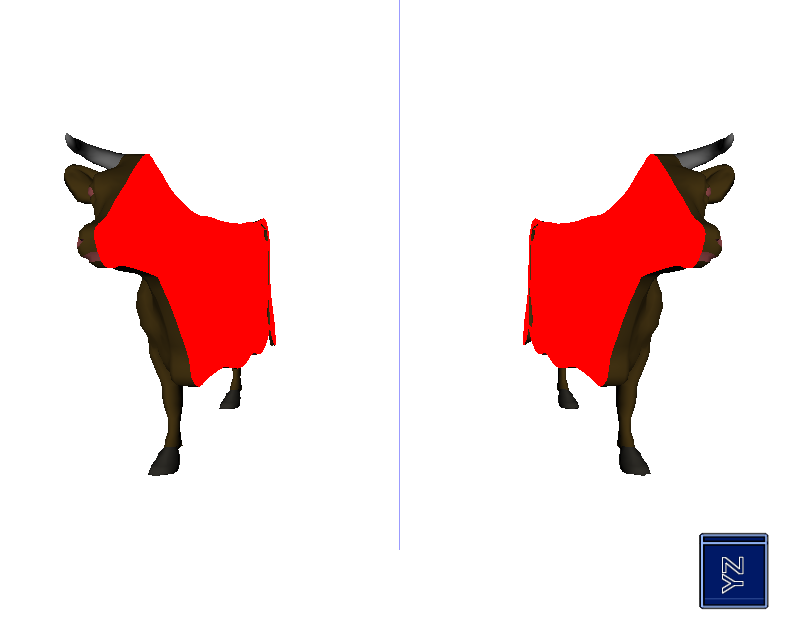
\includegraphics[width=0.4\textwidth]{ownChapters/figures/4_offset_flatInside.png}%
\hspace{7.00mm}
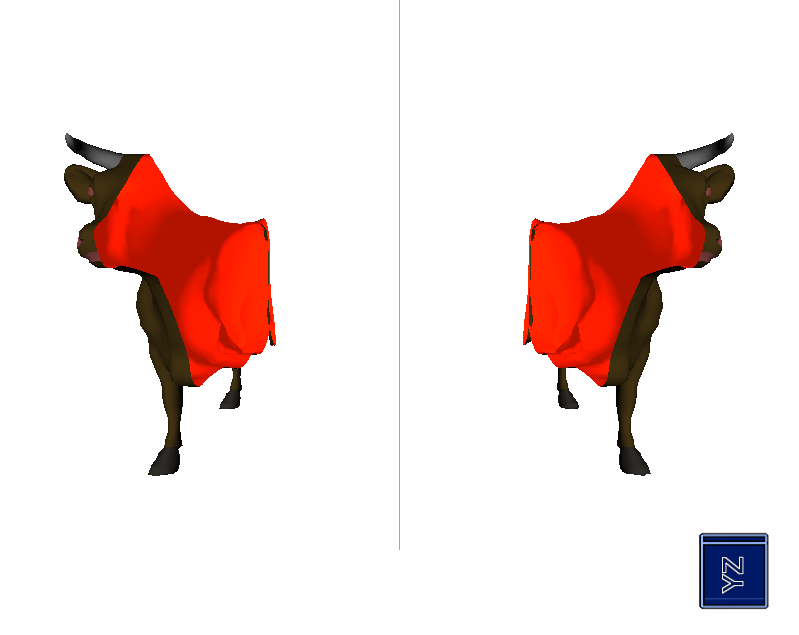
\includegraphics[width=0.4\textwidth]{ownChapters/figures/5_offset_phongInside.png}%
\hspace{7.00mm}
\includegraphics[width=0.4\textwidth]{ownChapters/figures/6_offset_paddedPhong.png}%
\caption{Different methods of shading the back faces (from upper left to lower right): no special treatment~\ref{fig:noInside}, flat shading, caved interior shading, cut surface shading.}%
\label{fig:shading}%
\end{figure}